\documentclass[]{book}
\usepackage{lmodern}
\usepackage{amssymb,amsmath}
\usepackage{ifxetex,ifluatex}
\usepackage{fixltx2e} % provides \textsubscript
\ifnum 0\ifxetex 1\fi\ifluatex 1\fi=0 % if pdftex
  \usepackage[T1]{fontenc}
  \usepackage[utf8]{inputenc}
\else % if luatex or xelatex
  \ifxetex
    \usepackage{mathspec}
  \else
    \usepackage{fontspec}
  \fi
  \defaultfontfeatures{Ligatures=TeX,Scale=MatchLowercase}
    \setmainfont[]{NanumGothic}
\fi
% use upquote if available, for straight quotes in verbatim environments
\IfFileExists{upquote.sty}{\usepackage{upquote}}{}
% use microtype if available
\IfFileExists{microtype.sty}{%
\usepackage{microtype}
\UseMicrotypeSet[protrusion]{basicmath} % disable protrusion for tt fonts
}{}
\usepackage{hyperref}
\hypersetup{unicode=true,
            pdftitle={삽화편두통 예방치료약물 진료지침},
            pdfauthor={대한두통학회 편두통진료지침위원회},
            pdfborder={0 0 0},
            breaklinks=true}
\urlstyle{same}  % don't use monospace font for urls
\usepackage{natbib}
\bibliographystyle{apalike}
\usepackage{longtable,booktabs}
\usepackage{graphicx,grffile}
\makeatletter
\def\maxwidth{\ifdim\Gin@nat@width>\linewidth\linewidth\else\Gin@nat@width\fi}
\def\maxheight{\ifdim\Gin@nat@height>\textheight\textheight\else\Gin@nat@height\fi}
\makeatother
% Scale images if necessary, so that they will not overflow the page
% margins by default, and it is still possible to overwrite the defaults
% using explicit options in \includegraphics[width, height, ...]{}
\setkeys{Gin}{width=\maxwidth,height=\maxheight,keepaspectratio}
\IfFileExists{parskip.sty}{%
\usepackage{parskip}
}{% else
\setlength{\parindent}{0pt}
\setlength{\parskip}{6pt plus 2pt minus 1pt}
}
\setlength{\emergencystretch}{3em}  % prevent overfull lines
\providecommand{\tightlist}{%
  \setlength{\itemsep}{0pt}\setlength{\parskip}{0pt}}
\setcounter{secnumdepth}{5}
% Redefines (sub)paragraphs to behave more like sections
\ifx\paragraph\undefined\else
\let\oldparagraph\paragraph
\renewcommand{\paragraph}[1]{\oldparagraph{#1}\mbox{}}
\fi
\ifx\subparagraph\undefined\else
\let\oldsubparagraph\subparagraph
\renewcommand{\subparagraph}[1]{\oldsubparagraph{#1}\mbox{}}
\fi

%%% Use protect on footnotes to avoid problems with footnotes in titles
\let\rmarkdownfootnote\footnote%
\def\footnote{\protect\rmarkdownfootnote}

%%% Change title format to be more compact
\usepackage{titling}

% Create subtitle command for use in maketitle
\providecommand{\subtitle}[1]{
  \posttitle{
    \begin{center}\large#1\end{center}
    }
}

\setlength{\droptitle}{-2em}

  \title{삽화편두통 예방치료약물 진료지침}
    \pretitle{\vspace{\droptitle}\centering\huge}
  \posttitle{\par}
    \author{대한두통학회 편두통진료지침위원회}
    \preauthor{\centering\large\emph}
  \postauthor{\par}
      \predate{\centering\large\emph}
  \postdate{\par}
    \date{2019-06-20}

\usepackage{booktabs}
\usepackage{amsthm}
\makeatletter
\def\thm@space@setup{%
  \thm@preskip=8pt plus 2pt minus 4pt
  \thm@postskip=\thm@preskip
}
\makeatother

\begin{document}
\maketitle

{
\setcounter{tocdepth}{1}
\tableofcontents
}
\frontmatter

\hypertarget{section}{%
\chapter*{머리말}\label{section}}
\addcontentsline{toc}{chapter}{머리말}

\hypertarget{section-1}{%
\chapter*{발간사}\label{section-1}}
\addcontentsline{toc}{chapter}{발간사}

김병건 회장님

\hypertarget{section-2}{%
\chapter*{간행사}\label{section-2}}
\addcontentsline{toc}{chapter}{간행사}

정재면 위원장님

\mainmatter

\hypertarget{section-3}{%
\chapter{요약본}\label{section-3}}

1. 성인 삽화편두통 환자에서 예방치료를 고려해야 하는 요인들(두통빈도, 두통강도, 환자의 선호도, 일상생활에 대한 영향 등)은 무엇인가?

\begin{itemize}
\item
  권고사항

  \begin{itemize}
  \tightlist
  \item
    삽화편두통에서 생활습관개선과 편두통 급성기치료를 적절하게 시도하였음에도 불구하고 편두통으로 인하여 의미 있는 일상생활의 장애\footnote{두통으로 인한 일상생활의 의미있는 장애(headache-related disability)

      신체적, 심리적, 사회경제적인 측면을 모두 포함하여 두통 환자가 겪게 되는 일상생활의 장애를 포괄적으로 의미하는 것이다. 즉, 두통으로 인한 신체적인 고통, 불안 또는 우울 등의 심리적 반응, 사회경제적인 비용의 증가, 학업 및 사회활동과 여가활동의 위축 등 삶의 질을 저하시키는 일체의 장애를 말한다. 예를 들면 아래와 같은 것이 있다.

      \begin{enumerate}
      \def\labelenumi{\arabic{enumi}.}
      \tightlist
      \item
        두통 때문에 학교나 직장을 결석 또는 결근(조퇴 또는 양호실에서 휴식)한 적이 있다.
      \item
        두통 때문에 학교나 직장에서 학습능률 또는 업무능력이 절반 이하로 감소한 적이 있다.
      \item
        학교나 직장을 다니지 않는 경우(예: 가정주부, 휴직 또는 퇴직), 두통 때문에 가사를 할 수 없었던 적이 있다.
      \item
        학교나 직장을 다니지 않는 경우(예: 가정주부, 휴직 또는 퇴직), 두통 때문에 가사능률이 절반 이하로 감소했던 적이 있다.
      \item
        두통 때문에 공휴일이나 근무시간 외에 가족활동, 사회활동, 또는 여가활동을 참여하지 못했거나 하였더라도 절반 이상의 불편함을 느낀 적이 있다.
      \end{enumerate}}를 겪는 경우에 예방치료를 권고한다. (근거수준: 전문가의견, 권고등급: 강함)
  \item
    편두통환자의 1)두통빈도(월 두통일수)가 적더라도 편두통 급성기치료를 하였을 때 편두통이 효과적으로 치료되지 않거나 두통으로 인한 장애를 경험하는 경우, 2)편두통 급성기치료가 효과적이더라도 두통빈도가 잦은 경우에 예방치료를 권고한다. (근거수준: 전문가의견, 권고등급: 강함)
  \item
    편두통환자가 편두통 급성기치료제를 월 10--15일 이상 사용하는 경우에 약물과용두통\footnote{\begin{longtable}[]{@{}lr@{}}
      \toprule
      편두통급성기치료제의 종류 & 약물과용두통 진단기준\tabularnewline
      \midrule
      \endhead
      에르고타민 & 월10일 이상 복용\tabularnewline
      트립탄 & 월10일 이상 복용\tabularnewline
      단순진통제(아세트아미노펜,아세틸살리실산) 또는 비스테로이드항염제(NSAIDs) & 월15일 이상 복용\tabularnewline
      마약성(opioid) 진통제 & 월10일 이상 복용\tabularnewline
      복합진통제 & 월10일 이상 복용\tabularnewline
      여러가지 종류의 약제를 혼용해서 복용하는 경우 & 월10일 이상 복용\tabularnewline
      \bottomrule
      \end{longtable}}의 우려가 있으므로 예방치료를 권고한다. (근거수준: 전문가의견, 권고등급: 강함)
  \item
    편두통환자의 두통빈도와 무관하게 편두통환자가 편두통 예방치료를 선호하는 경우이거나 담당의사가 임상적으로 예방치료가 필요하다고 판단하는 경우(예시: 뇌간조짐/반신마비편두통)에 예방치료를 고려할 수 있다. (근거수준: 전문가의견, 권고등급: 약함)
  \item
    편두통환자가 편두통 급성기치료의 의학적 금기를 가지고 있는 경우에 예방치료를 고려할 수 있다. (근거수준: 전문가의견, 권고등급: 약함)
  \end{itemize}
\end{itemize}

\begin{center}\rule{0.5\linewidth}{\linethickness}\end{center}

2. 성인 삽화편두통 환자에서 예방치료의 중단은 어떻게 결정해야 하는가?

\begin{itemize}
\item
  권고사항

  \begin{itemize}
  \tightlist
  \item
    삽화편두통에서 예방치료의 효능은 적정용량 혹은 최대내약용량(maximal tolerable dose)으로 적어도 2개월 이상 사용한 후 판단할 수 있다. (근거수준: 전문가의견, 권고등급: 약함)
  \item
    예방치료가 효과적인 경우 3개월 이상 치료를 지속한 후 용량을 감량하거나 중단하는 것을 시도할 수 있으며, 예방치료를 유지하는 기간은 두통의 빈도 및 강도 외에도 편두통이 일상 생활에 미치는 영향의 정도에 따라 환자마다 개별적으로 접근하는 것을 제안한다. (근거수준: 전문가의견, 권고등급: 약함)
  \item
    예방약물을 감량하거나 중단했을 때 편두통의 빈도가 증가하면 약물 용량을 증량하거나 다시 시작하기를 제안한다. (근거수준: 전문가의견, 권고등급: 약함)
  \item
    예방치료의 효능, 부작용 및 순응도를 평가하고 유지기간을 결정하기 위해서는 두통일기 작성을 권고한다. (근거수준: 전문가의견, 권고등급: 강함)
  \end{itemize}
\end{itemize}

\begin{center}\rule{0.5\linewidth}{\linethickness}\end{center}

3. 성인 삽화편두통 환자에서 예방치료로 베타차단제를 사용하는 것이 타약제, 위약 또는 치료하지 않는 것에 비해 두통의 완화에 효과적인가?

\begin{itemize}
\item
  권고사항

  \begin{itemize}
  \tightlist
  \item
    프로프라놀롤은 성인 삽화편두통 환자에서 편두통 예방약제로 사용하는 것을 권고한다. (근거수준: 높음, 권고등급: 강함)
  \item
    메토프롤롤은 성인 삽화편두통 환자에서 편두통 예방약제로 사용하는 것을 고려할 수 있다.(근거수준: 높음, 권고등급: 강함)
  \item
    아테놀롤은 성인 삽화편두통 환자에서 편두통 예방약제로 사용하는 것을 고려할 수 있다. (근거수준: 보통, 권고등급: 약함)
  \item
    나돌롤은 성인 삽화편두통 환자에서 편두통 예방약제로 사용하는 것을 고려할 수 있다. (근거수준: 보통, 권고등급: 약함)
  \item
    네비볼롤은 성인 삽화편두통 환자에서 편두통 예방약제로 사용하는 것을 고려할 수 있다. (근거수준: 낮음, 권고등급: 약함)
  \item
    비소프롤롤은 성인 삽화편두통 환자에서 편두통 예방약제로 사용하지 않을 것을 제안한다. (근거수준: U (낮음 or 전문가의견), 권고등급: 약함)
  \item
    핀돌롤은 성인 삽화편두통 환자에서 편두통 예방약제로 사용하지 않을 것을 제안한다. (근거수준: U (낮음 또는 전문가의견), 권고등급: 약함)
  \end{itemize}
\end{itemize}

\begin{center}\rule{0.5\linewidth}{\linethickness}\end{center}

4. 성인 삽화편두통 환자에서 예방치료로 칼슘통로차단제를 사용하는 것이 타약제, 위약 또는 치료하지 않는 것에 비해 두통의 완화에 효과적인가?

\begin{itemize}
\item
  권고사항

  \begin{itemize}
  \tightlist
  \item
    니카르디핀, 니페디핀, 니모디핀 등은 성인 삽화편두통 환자에서 편두통 예방약제로 사용하지 않을 것을 제안한다. (근거수준: 전문가의견, 권고등급: 약함)
  \item
    베라파밀은 성인 삽화편두통 환자에서 편두통 예방약제로 사용하지 않을 것을 제안한다. (근거수준: 전문가의견, 권고등급: 약함)
  \item
    플루나리진은 성인 삽화편두통 환자에서 편두통 예방약제로 사용하는 것을 고려할 수 있다. (근거수준: 높음, 권고등급: 약함)
  \item
    신나리진은 성인 삽화편두통 환자에서 삼환계 항우울제 및 베타차단제에 효과가 없거나 투여가 어려운 경우 편두통 예방약제로 사용하는 것을 고려할 수 있다. (근거수준: 낮음, 권고등급: 약함)
  \end{itemize}
\end{itemize}

\begin{center}\rule{0.5\linewidth}{\linethickness}\end{center}

5. 성인 삽화편두통 환자에서 예방치료로 안지오텐신수용체차단제(angiotensin receptor blocker)나 안지오텐신전환효소억제제(angiotensin-converting enzyme inhibitor)를 사용하는 것이 타약제, 위약 또는 치료하지 않는 것에 비해 두통의 완화에 효과적인가?

\begin{itemize}
\item
  권고사항

  \begin{itemize}
  \tightlist
  \item
    칸데사르탄은 성인 삽화편두통 환자에서 편두통 예방약제로 사용하는 것을 고려할 수 있다. (근거수준: 보통, 권고등급: 약함)
  \item
    리시노프릴은 성인 삽화편두통 환자에서 편두통 예방약제로 사용하는 것을 고려할 수 있다. (근거수준: 낮음, 권고등급: 약함)
  \item
    텔미사르탄은 성인 삽화편두통 환자에서 편두통 예방약제로 사용하지 않을 것을 권고한다. (근거수준: 낮음, 권고등급: 강함).
  \end{itemize}
\end{itemize}

\begin{center}\rule{0.5\linewidth}{\linethickness}\end{center}

6. 성인 삽화편두통 환자에서 예방치료로 항우울제를 사용하는 것이 타약제, 위약 또는 치료하지 않는 것에 비해 두통의 완화에 효과적인가?

\begin{itemize}
\item
  권고사항

  \begin{itemize}
  \tightlist
  \item
    아미트리프틸린은 성인 삽화편두통 환자에서 편두통 예방약제로 사용하는 것을 권고한다. (근거수준: 보통, 권고등급: 강함)
  \item
    벤라팍신은 성인 삽화편두통 환자에서 편두통 예방약제로 사용하는 것을 고려할 수 있다. (근거수준: 보통, 권고등급: 약함)
  \item
    플루옥세틴은 성인 삽화편두통 환자에서 편두통 예방약제로 사용하지 않을 것을 제안한다. (근거수준: 매우낮음, 권고등급: 약함)
  \item
    노르트리프틸린은 성인 삽화편두통 환자에서 편두통 예방치료제로 사용하는 것을 고려할 수 있다. (근거수준: 매우낮음, 권고등급: 약함)
  \end{itemize}
\end{itemize}

\begin{center}\rule{0.5\linewidth}{\linethickness}\end{center}

7. 성인 삽화편두통 환자에서 예방치료로 뇌전증약을 사용하는 것이 타약제, 위약 또는 치료하지 않는 것에 비해 두통의 완화에 효과적인가?

\begin{itemize}
\item
  권고사항

  \begin{itemize}
  \tightlist
  \item
    토피라메이트는 성인 삽화편두통 환자에서 편두통 예방약제로 사용할 것을 권고한다. (근거수준: 높음, 권고등급: 강함)
  \item
    디발프로엑스나트륨은 성인 삽화편두통 환자에서 편두통 예방약제로 사용할 것을 권고한다. 단, 체중 증가, 다낭성 난소 증후군 등의 부작용이 있어 여성에서 사용이 제한될 수도 있다. (근거수준: 높음, 권고등급: 강함) 발프로산은 성인 삽화편두통 환자에서 편두통 예방약제로 사용하는 것을 고려할 수 있다. (근거수준: 높음, 권고등급: 약함)
  \item
    가바펜틴은 성인 삽화편두통 환자에서 편두통 예방약제로 사용하지 않을 것을 제안한다. (근거수준: 매우낮음, 권고등급: 약함)
  \item
    레베티라세탐은 성인 삽화편두통 환자에서 편두통 예방약제로 사용하는 것을 고려할 수 있다. (근거수준: 낮음, 권고등급: 약함)
  \item
    조니사미드는 성인 삽화편두통 환자에서 편두통 예방약제로 사용하는 것을 고려할 수 있다. 토피라메이트가 가지고 있는 여러 부작용이 우려되고 다른 약제의 체중증가가 부담된다면 조니사미드를 고려해볼 수 있다. (근거수준: 낮음, 권고등급: 약함)
  \end{itemize}
\end{itemize}

\hypertarget{section-4}{%
\chapter{개요}\label{section-4}}

두통은 신경과 외래진료를 보게 되는 가장 흔한 증상으로, 평생 동안 전 인구의 70\% 이상이 두통을 경험하는 것으로 알려져 있다. 병원에 내원하는 두통환자에서 가장 흔한 원인은 편두통이며, 전 세계적 유병률은 10\% 내외로 추산되고 국내연구(Korean Headache Survey)에서 편두통 유병률은 6\% (남자 3\%, 여자 9\%)였다.

편두통 유병률은 사회경제적 활동이 보통 최고조에 이르는 30대부터 50대의 연령에서 높기 때문에, 편두통이 사회에 미치는 영향은 클 수 밖에 없다. 미국의 인구집단연구 결과에 따르면, 편두통으로 인해 학교 또는 직장에 결석하는 직접손실비용은 연간 10억 달러 이상이며, 학습이나 업무능률의 저하와 같은 간접손실비용은 연간 200억 달러에 달하는 것으로 조사되었다.

국제보건기구(World Health Organization)의 2013년도 세계질병부담연구(Global Burden of Disease 2013)에 따르면 편두통은 전체 질병에 의한 부담 중 7\%를 차지하고 전체질병 중에서 6번째로 장애를 유발하였다.

편두통은 대표적인 원발두통질환으로 과민한 뇌의 특성 그 자체로 인하여 두통이 발생하는 것으로 알려져 있다. 편두통을 임상적 특징으로 정의하면 발작적으로 발생하는 삽화성 경과의 두통과 함께 신경학적 증상의 동반을 반복적으로 경험하게 되는 만성 통증질환이다.

국제두통질환분류에서 편두통은 다양한 아형으로 정의될 수 있으며, 조짐여부에 따라 무조짐편두통과 조짐편두통으로 크게 구분하고 있다. 또한, 두통빈도에 따라 두통일수가 한 달에15일 이상이면서 그 기간이 3개월을 초과하는 경우에 만성편두통으로, 그 이하인 경우 삽화편두통으로 진단 분류된다. 삽화편두통 환자 중 일부는 만성편두통으로 진행되거나 삽화편두통 상태에서도 두통빈도의 악화 또는 급성기치료의 효율저하로 인하여 편두통으로 인한 일상생활의 장애(migraine-related disability)를 경험할 수 있다. 따라서, 삽화편두통 환자의 편두통 장애룰 감소시키기 위한 적절한 편두통예방치료의 전략이 필요하며, 임상현장에서는 이를 위해 참고할 편두통예방치료 진료지침이 필요하다. 삽화편두통의 경우 기존의 다양한 경구약물을 바탕으로 한 편두통예방치료의 근거와 국외진료지침이 있다. 따라서, 본 진료지침에서는 기존 및 최신의 근거를 체계적으로 고찰하고 국내의 삽화편두통 환자의 진료에서 활용이 가능한 편두통예방치료의 권고안을 제시하려 한다.

\cleardoublepage

\hypertarget{appendix-appendix}{%
\appendix}


\hypertarget{section-5}{%
\chapter{개발그룹}\label{section-5}}

\hypertarget{section-6}{%
\section{운영위원회}\label{section-6}}

\begin{itemize}
\tightlist
\item
  위원장: 인제대학교 정재면
\item
  간사: 중앙대학교 박광열
\end{itemize}

\hypertarget{section-7}{%
\section{자문위원회}\label{section-7}}

\begin{itemize}
\tightlist
\item
  을지대학교 김병건
\item
  연세대학교 김원주
\end{itemize}

\hypertarget{section-8}{%
\section{외부자문그룹}\label{section-8}}

\begin{itemize}
\tightlist
\item
  순천향대학교 이유경
\item
  NECA 박동아
\end{itemize}

\hypertarget{section-9}{%
\section{실무위원회및 근거평가그룹}\label{section-9}}

\begin{itemize}
\tightlist
\item
  분당제생병원 김병수
\item
  경북대학교 서종근
\item
  한림대학교 손종희
\item
  이화여자대학교 송태진
\item
  성균관대학교 이미지
\item
  성균관대학교 정필욱
\item
  NECA 최미영
\item
  전주예수병원 최윤주
\end{itemize}

\hypertarget{section-10}{%
\section{이해관계 선언}\label{section-10}}

운영위원회및 실무위원회의 모든 위원은 자문료, 연구비, 지적재산권드의 재정적 이해상충, 지적이해상충, 그리고 개인적 이해상충을 문서로 공개하였다.

\hypertarget{section-11}{%
\section{운영}\label{section-11}}

\hypertarget{section-12}{%
\subsection{합의원칙의 결정}\label{section-12}}

\begin{itemize}
\tightlist
\item
  토론
\end{itemize}

\hypertarget{section-13}{%
\subsection{저자원칙의 결정}\label{section-13}}

\begin{itemize}
\tightlist
\item
  초안:
\item
  최종보고서: 정재면
\item
  저자포함: 개발그룹전체
\end{itemize}

\hypertarget{section-14}{%
\subsection{잠재적 승인기구}\label{section-14}}

\begin{itemize}
\tightlist
\item
  대한두통학회
\item
  대한신경과학회
\end{itemize}

\hypertarget{section-15}{%
\subsection{보급전략}\label{section-15}}

\begin{itemize}
\tightlist
\item
  대한두통학회와 대한신경과학회 홈페이지 게시
\item
  대한두통학회지와 대한신경과학회지에 게재
\end{itemize}

\hypertarget{section-16}{%
\chapter{개발 계획}\label{section-16}}

\hypertarget{section-17}{%
\section{기존 진료지침 검색}\label{section-17}}

\begin{itemize}
\item
  Selection criteria

  -- From 2012 to 2016

  -- Written in English or Korean

  -- By Multi-disciplinary team

  -- Evidence-based method
\item
  9개의 진료지침 검토

  -- 2012 AAN AHS guideline update for migraine prophylaxis Neurology (김병수, 정필욱)

  -- 2012 Canadian guideline for migraine prophylaxis Can J neurol sci (이미지, 손종희)

  -- 2012 Croatia guideline (송태진, 손종희)

  -- 2012 Danish Guidelines JHP (서종근, 최윤주)

  -- 2012 French guidelines revised JHP (정필욱, 김병수)

  -- 2012 Italian Guidelines revised version -JHP supple (최윤주, 서종근)

  -- ICSI guideline 2013 (original version, full-text) (송태진, 김병수)

  -- NICE guideline for headache in over 12s (2012) (2015 update) (이미지, 김병건)

  -- Practice guideline update summary fot Botulinum neurotoxin (AAN) 2016 neurology (이미지)
\end{itemize}

\hypertarget{section-18}{%
\section{개발방법}\label{section-18}}

\begin{itemize}
\item
  Adaptation

  \begin{itemize}
  \item
    2012년까지의 진료지침 + 2012년 이후 논문은 핵심질문별로 다시 검색
  \item
    그외 수기로 논문 추가 조사 (논문의 참고문헌등)
  \end{itemize}
\end{itemize}

\hypertarget{section-19}{%
\chapter{범위결정과 핵심질문}\label{section-19}}

\hypertarget{section-20}{%
\section{범위결정}\label{section-20}}

\begin{itemize}
\item
  Population: Adult with frequent and/or moderate-to-severe episodic migraine
\item
  Intervention: Drug

  \begin{itemize}
  \tightlist
  \item
    Anti-epileptic drug
  \item
    Beta blocker/CCB/ARB/ACE
  \item
    Anti-Depressant
  \end{itemize}
\item
  Professional:

  \begin{itemize}
  \tightlist
  \item
    Primary care physician, Nurse, and healthcare professionals
  \end{itemize}
\item
  Outcome: The frequency of migraine prevention drug prescription as suggested
\item
  Healthcare setting: Primary care setting in Korea
\end{itemize}

\hypertarget{key-questions}{%
\section{Key Questions}\label{key-questions}}

\begin{enumerate}
\def\labelenumi{\arabic{enumi}.}
\item
  Episodic migraine환자에서 예방치료를 고려해야 하는 요인들(두통빈도, 두 통강도, 환자의 선호도, ADL에 대한 영향 등)은 무엇인가?
\item
  예방치료를 진행중인 episodic migraine환자에서 치료의 중단은 어떻게 결 정해야 하는가?
\item
  Episodic migraine환자에서 예방치료로 베타차단제(beta blocker: propranolol 등)를 사용하는 것이 타약제, 위약 또는 치료하지 않는 것에 비해 두통의 완화에 효과적인가?
\item
  Episodic migraine환자에서 예방치료로 칼슘채널차단제(calcium channel blocker: flunarizine 등)를 사용하는 것이 타약제, 위약 또는 치료하지 않는 것에 비해 두통의 완화에 효과적인가?
\item
  Episodic migraine환자에서 예방치료로 안지오텐신전환효소억제제(angiotensin converting enzyme inhibitor)나 안지오텐신수용체차단제(angiotensin receptor blocker: candesartan 등)를 사용하는 것이 타약제, 위약 또는 치료 하지 않는 것에 비해 두통의 완화에 효과적인가?
\item
  Episodic migraine환자에서 예방치료로 항우울제(anti-depressant: amitryptiline 등)를 사용하는 것이 타약제, 위약 또는 치료하지 않는 것에 비해 두통의 완화에 효과적인가?
\item
  Episodic migraine환자에서 예방치료로 항경련제(anti-epileptic agent: divalproex sodium, sodium valproate, topiramate 등)를 사용하는 것이 타약제, 위약 또는 치료하지 않는 것에 비해 두통의 완화에 효과적인가?
\end{enumerate}

\hypertarget{drugs}{%
\section{Drugs}\label{drugs}}

\begin{itemize}
\item
  Beta blocker

  \begin{itemize}
  \tightlist
  \item
    propranolol
  \item
    Metoprolol
  \item
    Timolol
  \item
    Atenolol
  \item
    Nadolol
  \item
    Nebivolol
  \item
    Pindolol
  \end{itemize}
\item
  Calcium channel blocker

  \begin{itemize}
  \tightlist
  \item
    flunarizine
  \item
    cinnarizine
  \item
    verapamil
  \item
    nicardipine
  \end{itemize}
\item
  angiotensin converting enzyme inhibitor or angiotensin receptor blocker

  \begin{itemize}
  \tightlist
  \item
    Lisinopril
  \item
    candesartan
  \end{itemize}
\item
  anti-depressant

  \begin{itemize}
  \tightlist
  \item
    amitryptiline
  \item
    nortriptyline
  \item
    Venlafaxine
  \item
    Fluoxetine
  \end{itemize}
\item
  anti-epileptic agent

  \begin{itemize}
  \tightlist
  \item
    divalproex sodium
  \item
    sodium valproate
  \item
    topiramate
  \item
    Carbamazepine
  \item
    Gabapentin
  \end{itemize}
\end{itemize}

\hypertarget{section-21}{%
\chapter{지침및 근거검색}\label{section-21}}

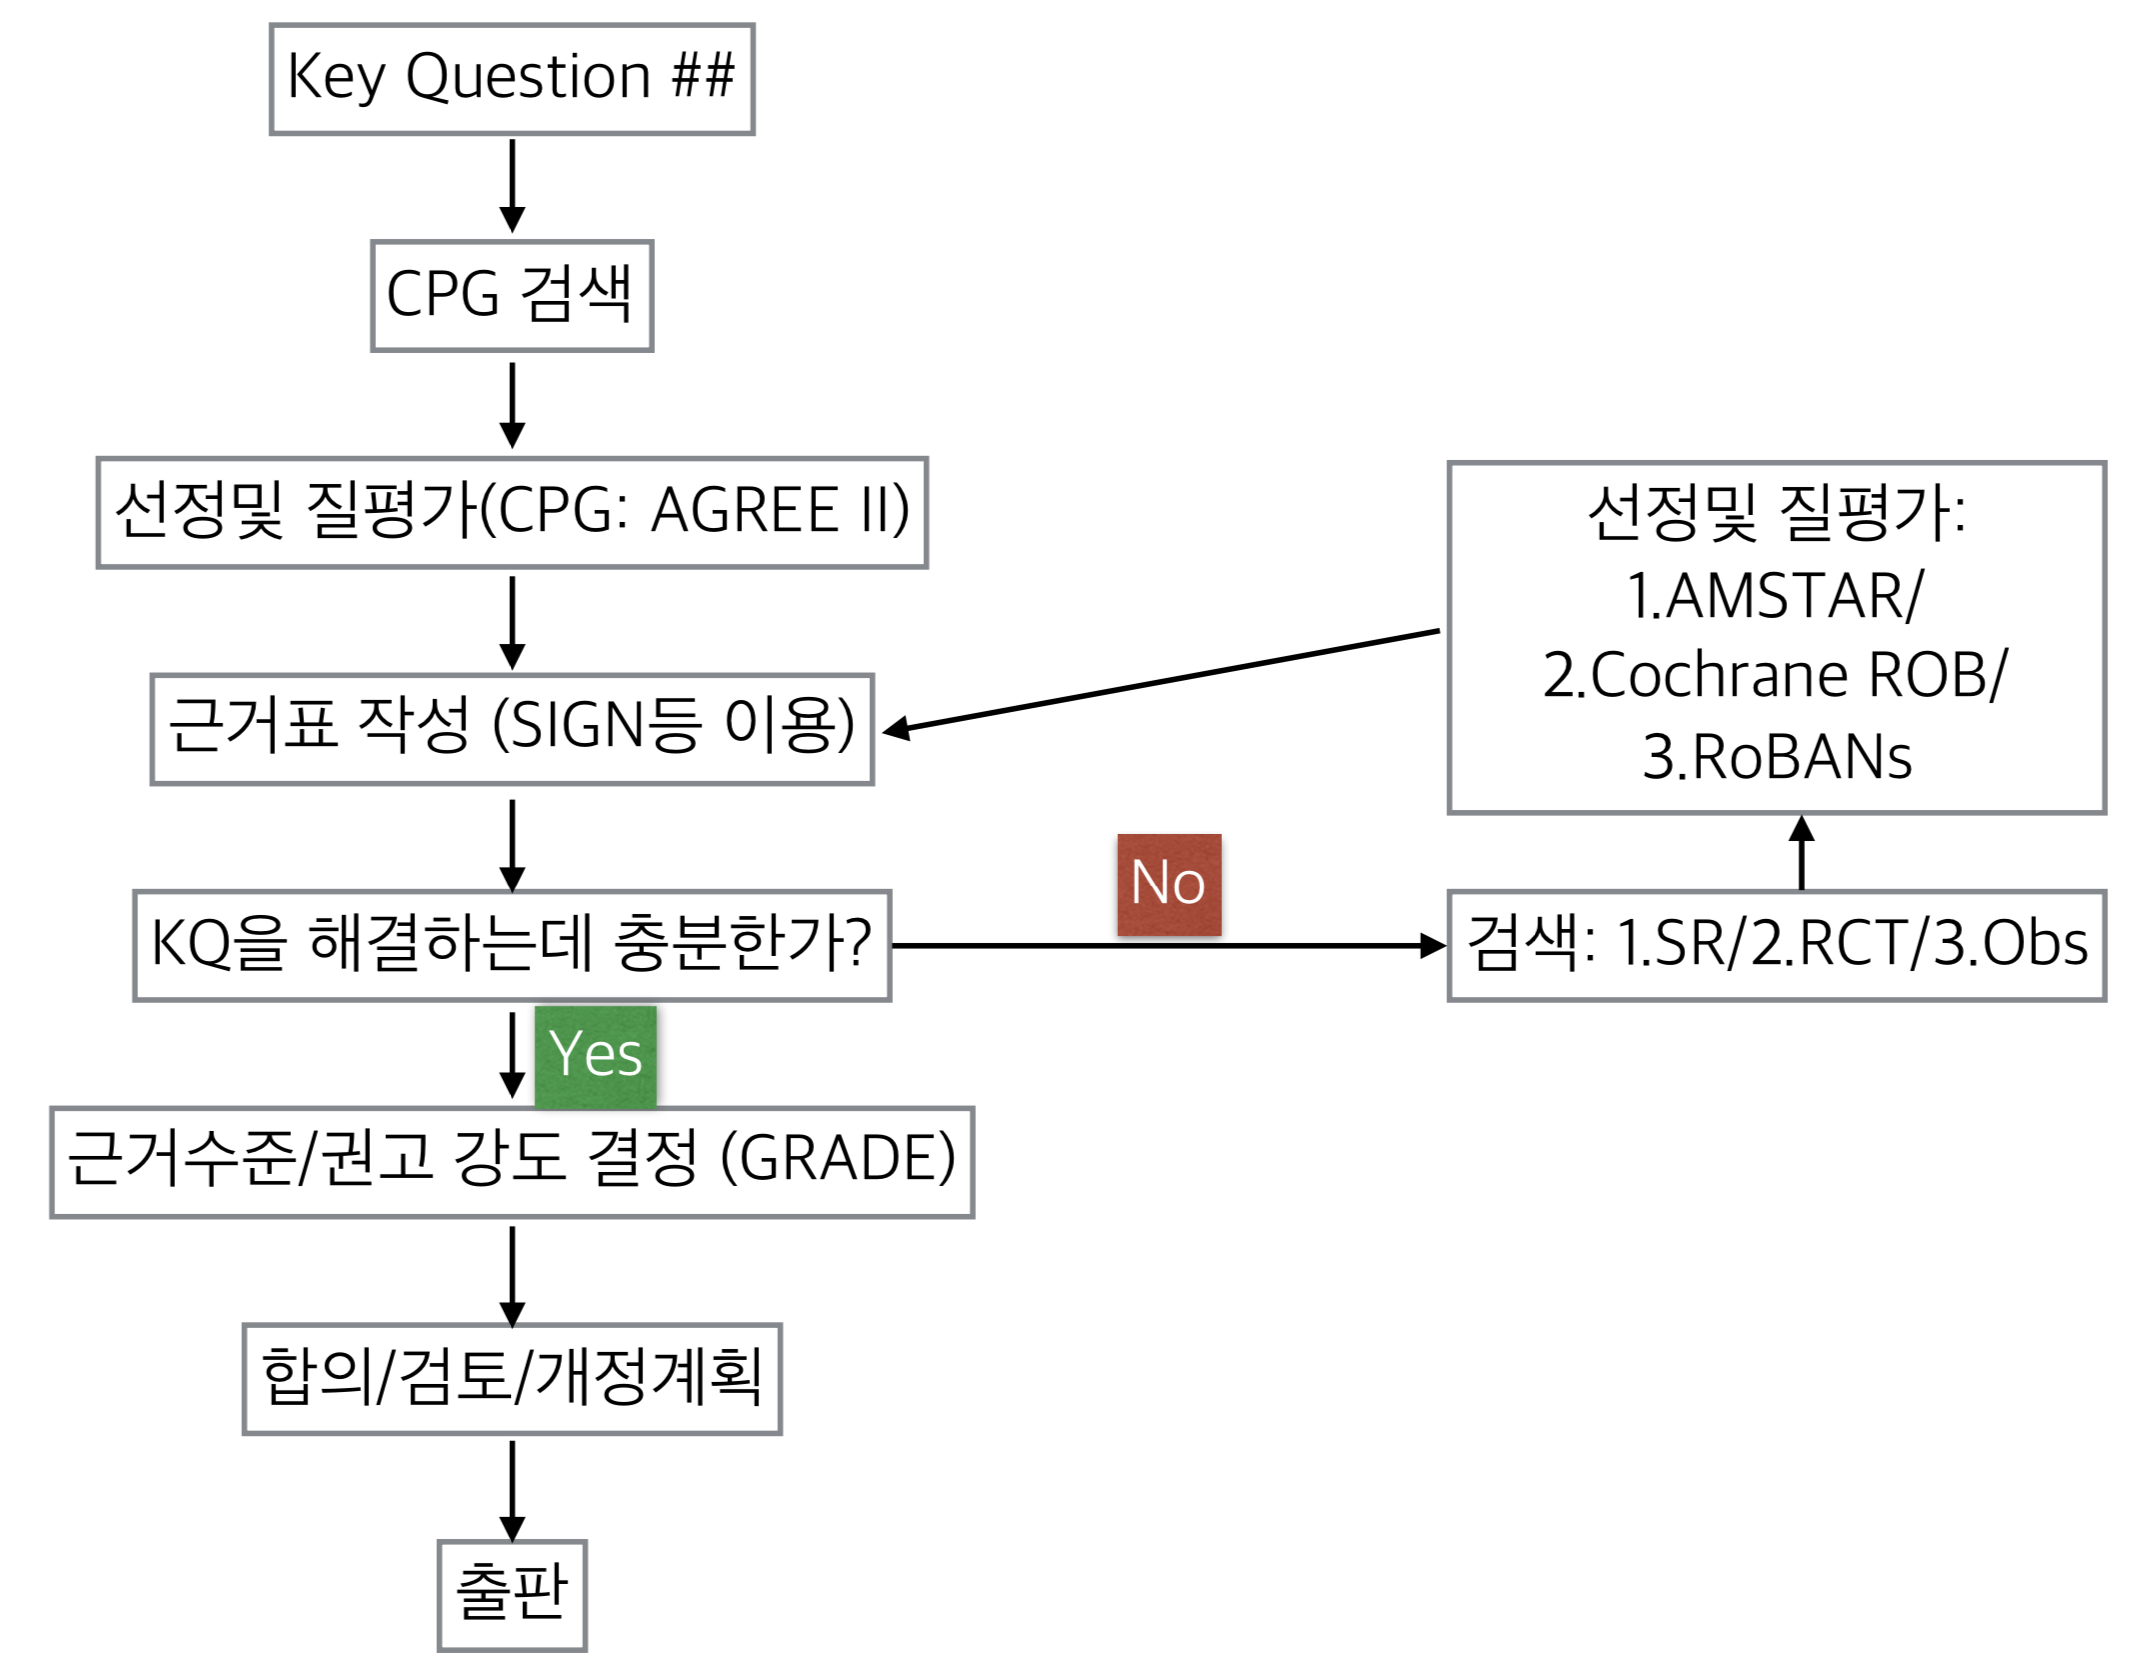
\includegraphics{static/SearchProcess.png}

\hypertarget{section-22}{%
\section{지침검색}\label{section-22}}

\begin{itemize}
\tightlist
\item
  National guideline clearinghouse
\item
  Guideline international network
\item
  Pubmed
\item
  Google search
\item
  KoMGI
\item
  KoreaMed - KMBASE
\end{itemize}

\hypertarget{section-23}{%
\section{근거검색}\label{section-23}}

\begin{itemize}
\item
  전자문헌검색:

  -상기 + Ovid DB(MEDLINE/EMBASE) Cochrane library
\item
  수기검색 (gray literature)
\end{itemize}

\hypertarget{section-24}{%
\section{핵심질문별 근거 평가자}\label{section-24}}

\begin{enumerate}
\def\labelenumi{\arabic{enumi}.}
\item
  Episodic migraine환자에서 예방치료를 고려해야 하는 요인들(두통빈도, 두 통강도, 환자의 선호도, ADL에 대한 영향 등)은 무엇인가?

  \begin{itemize}
  \tightlist
  \item
    김병수
  \end{itemize}
\item
  예방치료를 진행중인 episodic migraine환자에서 치료의 중단은 어떻게 결 정해야 하는가?

  \begin{itemize}
  \tightlist
  \item
    서종근
  \end{itemize}
\item
  Episodic migraine환자에서 예방치료로 베타차단제(beta blocker: propranolol 등)를 사용하는 것이 타약제, 위약 또는 치료하지 않는 것에 비해 두통의 완화에 효과적인가?

  \begin{itemize}
  \tightlist
  \item
    손종희
  \end{itemize}
\item
  Episodic migraine환자에서 예방치료로 칼슘채널차단제(calcium channel blocker: flunarizine 등)를 사용하는 것이 타약제, 위약 또는 치료하지 않는 것에 비해 두통의 완화에 효과적인가?

  \begin{itemize}
  \tightlist
  \item
    송태진
  \end{itemize}
\item
  Episodic migraine환자에서 예방치료로 안지오텐신전환효소억제제(angiotensin converting enzyme inhibitor)나 안지오텐신수용체차단제(angiotensin receptor blocker: candesartan 등)를 사용하는 것이 타약제, 위약 또는 치료 하지 않는 것에 비해 두통의 완화에 효과적인가?

  \begin{itemize}
  \tightlist
  \item
    이미지
  \end{itemize}
\item
  Episodic migraine환자에서 예방치료로 항우울제(anti-depressant: amitryptiline 등)를 사용하는 것이 타약제, 위약 또는 치료하지 않는 것에 비해 두통의 완화에 효과적인가?

  \begin{itemize}
  \tightlist
  \item
    정필욱
  \end{itemize}
\item
  Episodic migraine환자에서 예방치료로 항경련제(anti-epileptic agent: divalproex sodium, sodium valproate, topiramate 등)를 사용하는 것이 타약제, 위약 또는 치료하지 않는 것에 비해 두통의 완화에 효과적인가?

  \begin{itemize}
  \tightlist
  \item
    최윤주
  \end{itemize}
\end{enumerate}

\hypertarget{section-25}{%
\chapter{삽화성편두통 예방 진료지침}\label{section-25}}

\hypertarget{section-26}{%
\chapter{외부전문가 리뷰}\label{section-26}}

\hypertarget{section-27}{%
\chapter{지침 수정 계획과 발표}\label{section-27}}

\bibliography{book.bib,packages.bib}


\end{document}
